\begin{figure*}
\centering
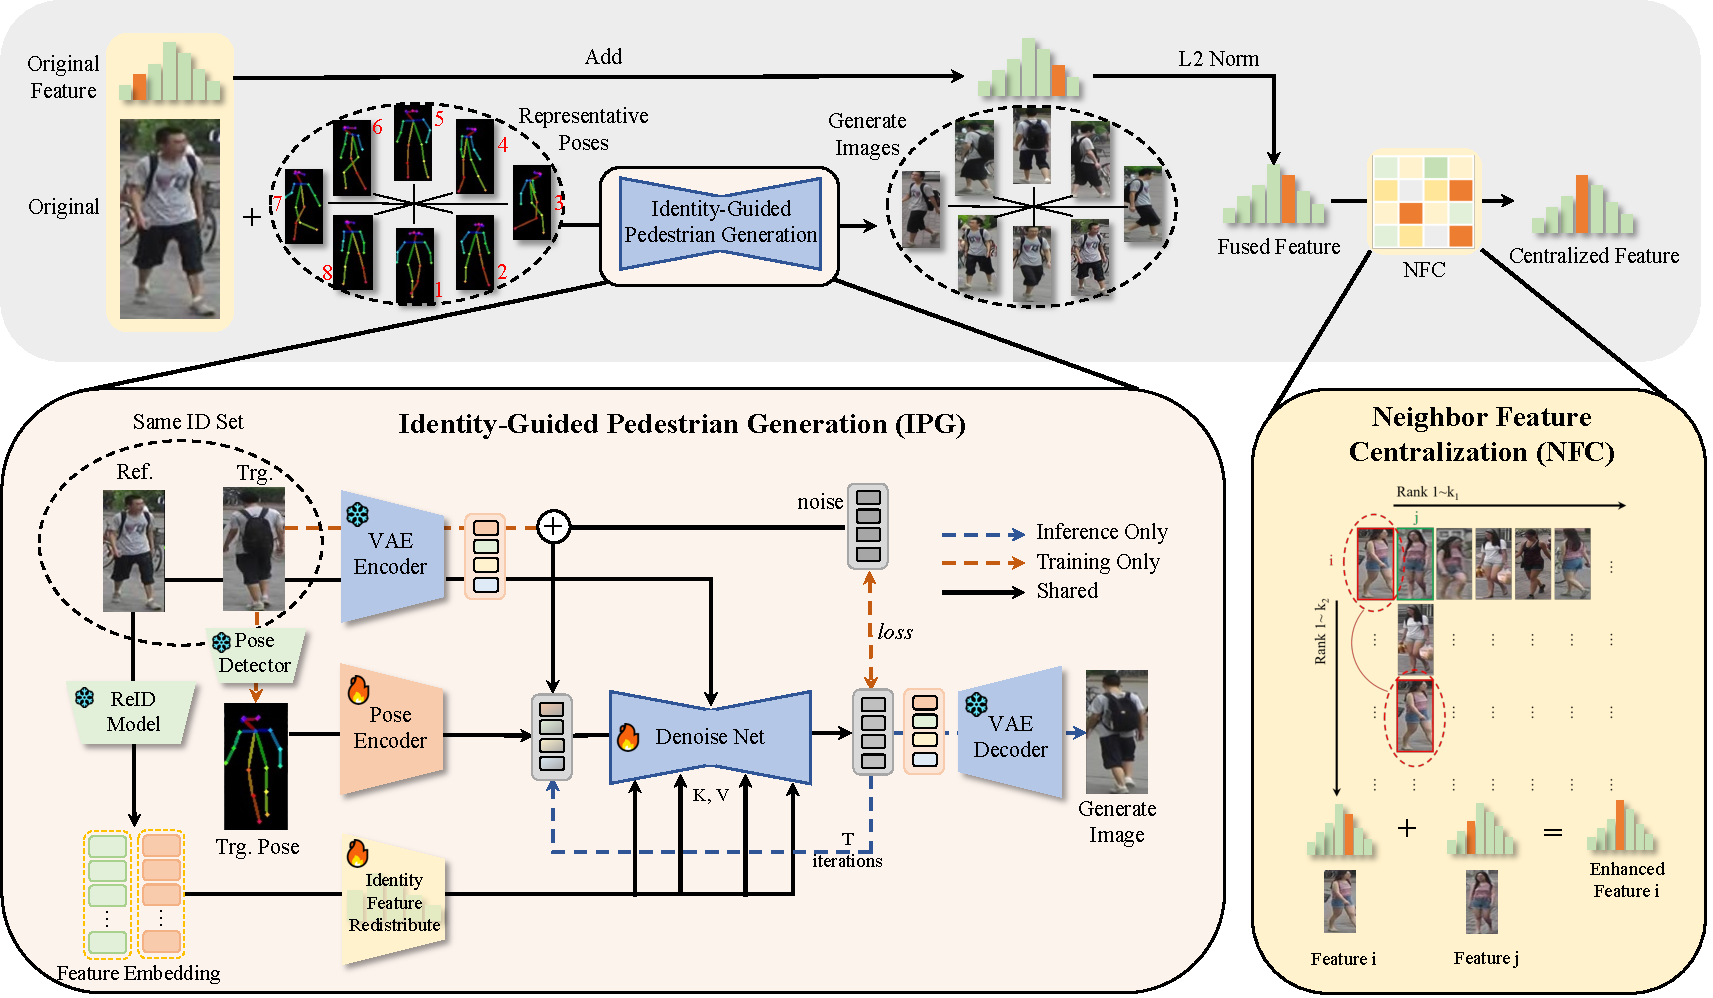
\includegraphics[width=0.85\textwidth]{figs/pdf/main.pdf}
\caption{Overview of the proposed Feature Centralization framework for the ReID task.}
\label{fig:main}
\end{figure*}

\section{Methods}
The main purpose of this paper is to \textbf{centralize features to their identity center} to enhance the identity representation of feature vectors extracted by ReID model, that is, reducing noise within the features while increasing the identity attributes to make them more representative of their identities. Therefore, to effectively and reasonably enhance the features, we need to understand the characteristics of the feature vectors obtained by ReID model.


\subsection{Feature Distribution Analysis} \label{Feature Distribution}

Currently, ReID models commonly use cross-entropy loss to impose ID-level constraints, and contrastive losses (such as triplet loss) to bring features of the same ID closer while pushing apart features of different IDs. Some models also utilize center loss to construct identity centers for dynamically constraining the IDs. These methods lead to one common result: feature aggregation. One can say that the current ReID task is essentially a feature aggregation task. The degree of feature density (e.g. t-SNE visualization) is also widely used to measure model performance. It is easy to deduce that the features of the same ID are centered around a "mean," approximately forming a normal distribution, as the distribution shown in Fig.\ref{fig:intro} which is visualized with one single feature dimension of the same ID.

It is evident that ReID features are normally distributed around the ‘identity center’. To theoretically prove that the feature vectors of each ID in current ReID tasks aggregation around a center or mean, we analyze several commonly used loss functions and their impact on the feature distribution in \textbf{Supplementary}.

For the same identity \( y_i = j \), we have a large number of samples \( \{\mathbf{x}_i\}_{i=1}^{N_j} \), where \( N_j \) is the number of samples for ID \( j \). These samples are passed through a ReID model \( f(\cdot) \), resulting in the corresponding feature vectors \( \{\mathbf{f}_i\}_{i=1}^{N_j} \):
\begin{equation}
\mathbf{f}_i = f(\mathbf{x}_i)
\end{equation}
where \( \mathbf{f}_i \in \mathbb{R}^d \) is the feature vector of sample \( \mathbf{x}_i \), and \( d \) is the dimensionality of the feature space.

For each feature dimension \( k \) of the feature vector \( \mathbf{f}_i \), the values \( \{\mathbf{f}_{i,k}\}_{i=1}^{N_j} \) obtained from different samples of the same ID \( j \) is independent and identically distributed random variables. Here, \( \mathbf{f}_{i,k} \) represents the \( k \)-th dimension of the feature vector for the \( i \)-th sample.

Since the input samples \( \{\mathbf{x}_i\}_{i=1}^{N_j} \) are independent, the values of \( \mathbf{f}_{i,k} \) are independent factors. According to the Central Limit Theorem (CLT), when the number of independent factors is large, the distribution of the values \( \{\mathbf{f}_{i,k}\}_{i=1}^{N_j} \) for any dimension \( k \) of the feature vector will approximate a normal distribution. Thus, for each feature dimension \( k \), we have:
\begin{equation}
\mathbf{f}_{i,k} \sim \mathcal{N}(\mu_k, \sigma_k^2)
\end{equation}
where \( \mu_k \) is the mean of the \( k \)-th feature dimension for ID f\( j \), and \( \sigma_k^2 \) is the variance of feature values in this dimension.

Since each dimension \( \mathbf{f}_{i,k} \) of the feature vector approximately follows a normal distribution across samples, the entire feature vector \( \mathbf{f}_i \) for ID \( j \) can be approximated by a multivariate normal distribution. This gives:
\begin{equation}
\mathbf{f}_i \sim \mathcal{N}(\boldsymbol{\mu}, \Sigma)
\end{equation}
where \( \boldsymbol{\mu} = (\mu_1, \mu_2, \dots, \mu_d)^\top \) is the mean vector of the feature dimensions, and \( \Sigma \) is the covariance matrix.

The theoretical analysis above suggests that under the optimization of the loss functions, the ReID model's feature vectors $\mathbf{x}_i$ aggregated around their identity centers $\mathbf{c}_{y_i}$ following a normal distribution. This is consistent with the feature aggregation observed in t-SNE visualizations.

\paragraph{Identity Density ($\text{ID}^2$) Metric}
Identity density is one aspect of measuring ReID effectiveness. However, there is currently no quantitative metric for this, and researchers commonly rely on visualization tools like t-SNE to demonstrate model performance. By using the concept above, we propose an Identity Density ($\text{ID}^2$) Metric which is detailed in \textbf{Supplementary}.
% That is,
% For a given identity \( y_i = i \), let \( \mathbf{z}_{i1}, \mathbf{z}_{i2}, \dots, \mathbf{z}_{in} \) represent the feature vectors extracted from different images of the same person. The mean feature vector \( \mathbf{\bar{z}}_i \), which serves as a more robust and representative feature for identity \( i \), can be computed as:
% \begin{equation}
% \mathbf{\bar{z}}_i = \frac{1}{n} \sum_{j=1}^{n} \mathbf{z}_{ij}
% \end{equation}

% In the ReID task, there are two main sets Gallery and Query, in the test of the dataset, is not allowed to utilize the a priori label information to assist in the recognition, which exists the information leakage, but in some particular scenarios, we may have multiple images of different poses or viewpoints of the searching target, it can be possible to overlay the features so that they are closer to the ID center to make it reduce the feature noise and be more ID representation.





% \subsection{Pose-based Pedestrians Generation}
\subsection{Feature Centralization via Identity-Guided Pedestrian Generation}

% In this section, we propose a novel method to centralize person features by generating images of the same individual (identity) with different poses using a Stable Diffusion model guided by identity feature. This approach leverages the conclusion above that features of the same identity follow a normal distribution, allowing for direct aggregation to centralize features to fit the identity center.

% Our purpose is to generate diverse images of a person under different poses and use these images to improve the feature representation of that person. 
\subsubsection{Feature Centralization}

Since features of the same identity follow a multivariate normal distribution, we can simply \textbf{aggregate features of the same identity to approximate the identity center}, as the visualization in Fig.\ref{fig:intro}. Thus, our main purpose becomes how to get more samples of the same identity to help centralize features.

\label{flip}
A straightforward approach is to perform horizontal flipping on the original images, and add features together. It is worth noting for reviewers that this is a very simple but effective trick. Therefore, it is necessary to check whether performance improvements are due to such tricks. In our experiments, to demonstrate the advancement of our approach, we did not use this trick. If used, it may be better. 

\subsubsection{Identity-Guided Diffusion Process}
To get more samples from the same identity, we propose a novel Identity-Guided Pedestrian Generation (IPG) paradigm, generating images of the same identity with different poses using a Stable Diffusion model guided by identity feature to centralize each sample's features. 
 
Followed by Stable Diffusion \cite{rombach2022high}, which is developed from latent diffusion model (LDM). We use the reference UNet to inject the reference image features into the diffusion process with a constant timestep \( t = 0 \), and the denoising UNet $\boldsymbol{\epsilon}_{\theta}$ to generate the target image latent \(\mathbf{z_0} \) by denoising the noisy latent \( \mathbf{z_T} = \boldsymbol{\epsilon}\):
\begin{equation}
\mathbf{z}_{t-1}=\boldsymbol{\epsilon}_{\theta}(\mathbf{z}_t, t, \mathbf{E}_{\text{pose}}, \mathbf{H}), t \in [0,T]
\end{equation}
where \( \mathbf{H} \) is the identity feature information to guide model keep person identity. \( \mathbf{E}_{\text{pose}} \) is the pose features.

At each timestep \( t \), the pose feature \( \mathbf{E}_{\text{pose}} \) and conditioning embedding \( \mathbf{H} \) guide the denoising process.
\\
\textbf{Identity Feature Redistribute (IFR)}
The Identity Feature Redistribute (IFR) module aims to utilize identity features from input images, removing noise to better guide the generative model. It converts high-dimensional identity features into meaningful low-dimensional feature blocks, enhancing the model’s feature utilization efficiency.

Given the input sample $\mathbf{x} \in \mathbb{R}^{C}$ by a ReID model \( f(\cdot) \), with IFR, we can obtain a re-distributed robust feature $\mathbf{H}\in \mathbb{R}^{N \times D})$ :
\begin{gather}
\mathbf{H} = \text{IFR}(f(\mathbf{x})) = \text{LN}(\text{Linear}(\mathbf{f}))
\end{gather}

For this more robust feature identity feature, it is used as the K, V of the model's attention module to guide the model's attention to the identity feature.
\\
\textbf{Pose Encoder}
The Pose Encoder is to extract high-dimensional pose embeddings $\mathbf{E}_{\text{pose}}$ from input poses. It has 4 blocks with 16,32,64,128 channels. Each block applies a normal \(3 \times 3\) Conv, a \(3 \times 3\) Conv with stride 2 to reduce spatial dimensions, and followed by a SiLU activate function. Subsequently, the pose features are added to the noise latent before into the denoising UNet, follows \cite{hu2024animate}.
\\
\textbf{Training Strategy}
For each identity $i$, we randomly select one image from \( S_i^{\text{ref}} \) as the reference image and one image from \( S_i^{\text{trg}} \) as the target image for training.

Let \( \mathbf{x}_{i,j}^{\text{ref}} \in S_i^{\text{ref}} \) denote the reference image (i.e. $j_{th}$ image of the $i_{th}$ ID) and \( \mathbf{x}_{i,j}^{\text{trg}} \in S_i^{\text{trg}} \) denote the target image. Model is trained using the mean squared error (MSE) loss between the predicted noise and the true noise.
\begin{equation}
\mathcal{L} = \mathbb{E}_{\mathbf{z}, t, \boldsymbol{\epsilon}} \left[ \left\| \boldsymbol{\epsilon} - \boldsymbol{\epsilon})\theta(\mathbf{z}_t, t, \mathbf{E}_{\text{pose}}, \mathbf{H}) \right\|^2 \right]
\end{equation}
where $\mathbf{z}=\text{VAE}(\mathbf{x}^{\text{trg}}_{i,j})+\boldsymbol{\epsilon}$ is a latent obtained by a pre-trained VAE encoder\cite{kingma2013auto}, $\mathbf{E}_{\text{pose}}$ is the pose feature of $\mathbf{x}^{\text{trg}}_{i,j})$, $\mathbf{H}$ is the re-distributed identity feature of $(\mathbf{x}^{\text{ref}}_{i,j}))$.

The model is trained to learn the mapping from the reference image \( \mathbf{x}_{\text{ref}} \) to the target image \( \mathbf{x}_{\text{trg}} \), with the goal of generating realistic variations in pose while preserving identity feature. This random selection ensures diversity during training, as different combinations of reference and target images are used in each training iteration, enhancing the model’s ability to generalize across various poses and viewpoints.


\subsubsection{Selection of Representative Pose} \label{standard pose}

In ReID tasks, features extracted from different poses of the same identity can vary significantly. Some specific poses tend to be more representative of that identity. As the conclusion of feature distribution in section\ref{Feature Distribution}, we calculate the identity center for IDs with all of its samples in datasets, and select the image whose feature is the closest to the center. The pose of this image is regarded as the representative pose. By randomly selecting 8 representative poses with different directions, we generate images that are more representative of the person’s identity.

That is, given a set of feature vectors \( \mathbf{F}_{\text{all}} = \{ \mathbf{f}_1, \mathbf{f}_2, \dots, \mathbf{f}_N \} \) for a particular identity:
\begin{equation}
\mathbf{f}_{\text{mean}} = \frac{1}{N} \sum_{i=1}^{N} \mathbf{f}_i
\end{equation}
\begin{equation}
\text{pose} = \arg \min_{i}d(\mathbf{f}_{\text{mean}}, \mathbf{f}_i) 
\end{equation}

% Theoretically, the more poses we aggregate, the closer the generated features will be to the identity center \( \mathbf{f}_{\text{mean}} \). However, it is impossible to generate an image that perfectly resembles the true appearance in all aspects. For instance, a back-facing image cannot realistically generate the front-side pattern of a shirt. Using such generated images may introduce additional noise into the model, which can be detrimental, particularly for models sensitive to local features.

% To address this issue, we designed a parameter-free, fast, and simple pose similarity algorithm. This algorithm selects the top \( M \) "standard poses" that are most similar to the reference pose, thereby reducing the noise caused by generating images from poses that differ significantly from the reference.

% First, normalize the input poses to eliminate scale differences. Let \( \mathbf{p} \) represent the keypoints of a pose. The height of the body is defined as the Euclidean distance between the neck keypoint \( \mathbf{p}_1 \) and the pelvis keypoint \( \mathbf{p}_{11} \), because the length of a person's body as well as the position of the neck is relatively fixed when walking.
% \begin{equation}
% h_{\text{body}} = \left\| \mathbf{p}_1 - \mathbf{p}_{11} \right\|
% \end{equation}
% \begin{equation}
% \hat{\mathbf{p}} = \frac{\mathbf{p} - \mathbf{p}_1}{h_{\text{body}}}
% \end{equation}

% To compare two poses \( \mathbf{p}_1 \) and \( \mathbf{p}_2 \), we first normalize both poses as described above. The similarity between the poses is then computed as the sum of the Euclidean distances between corresponding keypoints:
% \begin{equation}
% \text{similarity}(\hat{\mathbf{p}}_1, \hat{\mathbf{p}}_2) = \sum_{i=1}^{K} \left\| \hat{\mathbf{p}}_1^i - \hat{\mathbf{p}}_2^i \right\|
% \end{equation}
% where \( K \) is the number of keypoints in the pose, and in this paper \( K = 18\) follows DWpose\cite{yang2023effective}

% In this method, we begin by generating \( N \) standard poses for a given identity based on feature similarity to the identity's feature center. However, not all poses are equally beneficial for feature enhancement. Some poses may introduce significant noise, especially if they are vastly different from the reference pose. To mitigate this, we select the top \( M \) most similar poses from the \( N \) generated poses based on their similarity to the reference pose.
% \begin{equation}
% \text{Top-M} = \arg \min_{i \in [1, N]} \text{similarity}(\mathbf{p}_{\text{ref}}, \mathbf{p}_i)
% \end{equation}

\subsubsection{Feature Centralization Enhancement}
Once we got generated images with different poses, we generate new images \( \hat{\mathbf{x}} \) for each of these poses. The features extracted from these generated images are then aggregated with the original reference feature to enhance the overall representation. The centralized feature \(\tilde{\mathbf{f}}\) is computed as:
\begin{equation}
\tilde{\mathbf{f}}  = \|\mathbf{f} + \frac{\eta}{M} \sum_{i=1}^{M} \mathbf{f}_{i}\|_2
\end{equation}
where \( \mathbf{f}\) is the feature of the original reference image, and \( \mathbf{f}_{i} \) are the features extracted from the \( M \) generated images. The coefficient \( \eta \) is introduced to adjust based on the quality of generated images. According to the theory of Section\ref{Feature Distribution}, low-quality generated images, as long as they contain corresponding identity information, can also be applied with feature enhancement, and use \( \eta \) to regulate the enhancement effect of generated information. As discussed in \cite{zheng2017unlabeled}, even if quality is poor, it still contains ID information.

% This strategy ensures that generated images contribute to feature aggregation without introducing significant discrepancies, particularly for models that are sensitive to part details. By focusing on the most similar poses and aggregating their features, we can create a more robust and representative feature for each sample.
\subsection{Neighbor Feature Centralization (NFC)}

Moreover, we proposed a \textbf{Neighbor Feature Centralization (NFC)} algorithm to reduce noise in individual features and improve their identity discriminability in unlabeled scenarios. The core idea of the algorithm is to utilize mutual nearest-neighbor features for aggregation. 
% It still focuses on the main purpose of this paper: \textbf{utilize as much as the poses have for ID Representation}. 
\begin{algorithm}[H]
\caption{Neighbor Feature Centralization (NFC)}
\label{alg:feature_enhancement}
\begin{algorithmic}[1] 
\Require Feature vectors \(\{\mathbf{z}_i\}_{i=1}^N\), parameters \(k_1\), \(k_2\)
\Ensure Centralized feature vectors \(\{\mathbf{z}_i^{\text{centralized}}\}_{i=1}^N\)

\State Compute pairwise distance matrix \(\mathbf{D} = [d_{ij}]\)
\For{\(i = 1\) to \(N\)}
    \State Set \(d_{ii} = C\) \Comment{Avoid self-matching}
\EndFor
\For{\(i = 1\) to \(N\)}
    \State \(\mathcal{N}_{i} \gets\) indices of top \(k_1\) neighbors of \(\mathbf{z}_i\)
\EndFor
\For{\(i = 1\) to \(N\)}
    \State \(\mathcal{M}_{i} \gets \emptyset\)
    \For{each \(j \in \mathcal{N}_{i}\)}
        \State \(\mathcal{N}_{j}^{k_2} \gets\) indices of top \(k_2\) neighbors of \(\mathbf{z}_j\)
        \If{\(i \in \mathcal{N}_{j}^{k_2}\)}
            \State \(\mathcal{M}_{i} \gets \mathcal{M}_{i} \cup \{ j \}\)
        \EndIf
    \EndFor
\EndFor
\For{\(i = 1\) to \(N\)}
    \State \(\mathbf{z}_i^{\text{centralized}} \gets \mathbf{z}_i + \sum_{j \in \mathcal{M}_{i}} \mathbf{z}_j\)
\EndFor
\end{algorithmic}
\end{algorithm}
By enhancing each feature with its potential neighbors, it could effectively approximate features of the same identity without explicit labels, and ensure that only features have high similarity relationships contribute to the enhancement.

% \section{}





